\chapter{METODOLOGÍA} 
\section{ Método, tipo y nivel de investigación}

\subsection{Método de la investigación}
En esta investigación, se empleará el Método Científico como enfoque general. Específicamente, se utilizará un método Observacional, Transversal y Analítico para llevar a cabo el estudio \cite{popper1934}.

\subsection{Tipo de Investigación}

En esta investigación se ha realizado un estudio observacional, prospectivo, descriptivo y transversal para evaluar la calidad del agua en la Laguna de Pacucha. Según Supo \cite{supo2020} un estudio observacional implica que los datos se recogen sin manipular el entorno. En un estudio prospectivo, se recopilan datos actuales y futuros, proporcionando un control en el momento de la recolección. El enfoque descriptivo se centra en describir las características y condiciones de la laguna, mientras que el diseño transversal implica la recopilación de datos en un único punto en el tiempo, ofreciendo una instantánea de las condiciones actuales.

\subsection{Nivel de la Investigación}

Esta investigación abarca dos niveles: descriptivo y predictivo. Un estudio descriptivo se centra en proporcionar una descripción detallada de fenómenos, hechos o eventos en un campo específico del conocimiento, caracterizando de manera precisa las variables de interés. Este nivel de investigación no pretende establecer relaciones causales, sino ofrecer una visión clara y precisa de las condiciones actuales. Por otro lado, un estudio predictivo se enfoca en desarrollar modelos matemáticos para calcular la probabilidad de ocurrencia de un fenómeno, hecho o evento específico. Esto requiere un conocimiento previo de las causas que lo provocan. A diferencia del nivel explicativo, en el nivel predictivo, las causas ya son conocidas, por lo que el investigador puede desarrollar la intervención o crear un modelo predictivo a partir de una intervención donde no tuvo participación \cite{supo2020}.

En el contexto de esta investigación sobre la calidad del agua en la Laguna de Pacucha, se emplearán tanto el nivel descriptivo como el predictivo. El nivel descriptivo se utilizará para evaluar y caracterizar los parámetros fisicoquímicos del agua, como el oxígeno disuelto, el pH y la temperatura, proporcionando una imagen detallada de la calidad del agua en la laguna. Simultáneamente, se aplicará el nivel predictivo mediante análisis geoestadísticos para modelar y predecir la distribución espacial de estos parámetros en la laguna. Así, esta investigación no solo describe el estado actual del agua, sino que también anticipa posibles cambios y áreas problemáticas, orientando acciones de conservación y gestión efectiva.


\subsection{ Diseño de la investigación}
La investigación se llevará a cabo utilizando un enfoque comparativo que combina características observacionales, retrospectivas, transversales y analíticas \cite{shadish2002experimental}. En este estudio, se analizarán los parámetros fisicoquímicos de la Laguna de Pacucha y se compararán con los estándares de calidad de agua establecidos en Perú. Esta metodología posibilitará una evaluación precisa de la calidad del agua en la laguna, ofreciendo un marco de referencia claro y ampliamente reconocido. Al contrastar los resultados con las normativas nacionales, se podrá determinar si la calidad del agua en la Laguna de Pacucha cumple con los requisitos necesarios para su utilización y conservación. Este enfoque de investigación garantiza que los descubrimientos sean pertinentes y aplicables en el contexto peruano, lo que facilita la implementación de medidas adecuadas basadas en las conclusiones obtenidas.

\section{Materiales y Métodos}

\subsection{Materiales Utilizados}

Para llevar a cabo este estudio sobre estimación de los parámetros fisicoquímicos de la calidad del agua en la Laguna de Pacucha, se emplearon dos instrumentos esenciales para asegurar la precisión y fiabilidad de los datos recolectados.

El primero fue un avanzado multiparámetro de la marca Hanna, modelo HI98194. Este dispositivo es fundamental en la investigación de campo, ya que puede medir simultáneamente y con alta precisión parámetros fisicoquímicos críticos como el pH, la temperatura y el oxígeno disuelto. Estas mediciones son cruciales para una evaluación  del estado y la calidad del agua de la laguna.

El segundo instrumento clave fue un GPS de alta precisión de la marca Garmin, modelo 65s. Este dispositivo se utilizó para determinar con precisión las coordenadas geográficas exactas de cada punto de muestreo. Esto es esencial para correlacionar las mediciones fisicoquímicas con su ubicación específica y asegurar la reproducibilidad de la investigación.

\subsubsection{Multiparámetro Hanna HI98194}
Este avanzado instrumento se empleó para medir in situ diversos parámetros fisicoquímicos del agua, incluyendo temperatura, pH, oxígeno disuelto y conductividad. La precisión y la capacidad de realizar mediciones simultáneas de varios indicadores aseguran una evaluación exhaustiva y confiable de la calidad del agua en cada punto de muestreo.

\subsubsection{GPS Garmin 65s}
Para garantizar la exactitud en la localización de los puntos de muestreo, se utilizó este dispositivo GPS de alta precisión. Al permitir registrar las coordenadas geográficas exactas de cada punto, facilita la reproducibilidad del estudio y la correlación precisa de los datos fisicoquímicos con su ubicación específica en la laguna.

\subsection{Procedimiento}

\subsubsection{Preparación del Terreno y Muestreo}
El proceso comenzó con una cuidadosa planificación utilizando Google Maps para localizar la Laguna de Pacucha y diseñar una cuadrícula semi-regular en el mapa. Esta cuadrícula fue esencial para seleccionar estratégicamente los puntos de muestreo, representando adecuadamente la diversidad de condiciones dentro de la laguna. Una vez definidos los puntos, se imprimió un mapa detallado de la Laguna de Pacucha para su uso en el campo.



Posteriormente, recolectaron datos fisicoquímicos como la temperatura, el pH y el oxígeno disuelto utilizando el medidor multiparamétrico Hanna HI98194. En cada punto, el instrumento se sumergió hasta una profundidad de 50 cm, una norma establecida para obtener una muestra representativa de la masa de agua. El equipo midió meticulosamente el pH, la temperatura y el oxígeno disuelto, registrando cada valor con precisión para su posterior análisis. También tomaron notas detalladas sobre las condiciones ambientales y las características visuales del entorno, proporcionando un contexto más amplio para interpretar los datos fisicoquímicos.

Este procedimiento se repitió rigurosamente en cada uno de los puntos de muestreo establecidos en la cuadrícula de la laguna Pacucha. Esta sistemática garantizó una cobertura completa y representativa de la laguna, permitiendo una evaluación detallada de la calidad de sus aguas. Los datos recogidos son esenciales para realizar un análisis en profundidad, que se espera revele patrones significativos, tendencias y áreas potenciales de preocupación respecto a la calidad del agua de la laguna.

% Los métodos y materiales descritos en esta sección son el pilar fundamental de este estudio sobre la Laguna de Pacucha. La utilización de tecnología avanzada y un enfoque metódico en el muestreo garantiza que los resultados obtenidos no solo sean precisos y representativos, sino que también ofrezcan una visión profunda del estado actual y las dinámicas de la calidad del agua en este valioso ecosistema acuático. Estos datos proporcionarán una base sólida para futuros análisis, decisiones de gestión y estrategias de conservación.


\section{Población y muestra}
\subsection{Población}

 La población objeto de estudio en este estudio fue la laguna de Pacucha, ubicada en el distrito de Pacucha, provincia de Andahuaylas.
 Con una extensión aproximada de 7 km², esta laguna posee una importante biodiversidad y desempeña un papel crucial en el ecosistema local. Para garantizar la representatividad de la población, se adoptó una metodología basada en los principios de las normas internacionales, como la ISO 3951 -1:2005. Utilizando Google Maps y GPS, se seleccionaron 35 puntos de muestreo sistemático en una cuadrícula regular que cubría toda la laguna. Este enfoque garantizó una cobertura uniforme de la laguna y facilitó la comparación de los resultados obtenidos en diferentes áreas. La aplicación de esta metodología en la laguna de Pacucha es significativa, ya que proporciona una base sólida para la recogida de muestras de agua y el análisis de los parámetros fisicoquímicos, lo que permite obtener una imagen representativa de la calidad del agua en la laguna.

 

 Para evaluar los parámetros físico-químicos de la Laguna de Pacucha, se delimita como población de estudio el conjunto de características fisicoquímicas del agua distribuidas en toda la laguna. La calidad del agua y sus variaciones espaciales son el objeto central de este estudio, enfocándose en elementos como la temperatura, pH, oxígeno disuelto, conductividad, turbidez, entre otros, que son indicativos de la salud y calidad del ecosistema acuático.

El muestreo se realizó en 35 puntos estratégicamente distribuidos a lo largo de la Laguna de Pacucha. Para garantizar la precisión y fiabilidad de los datos recolectados, se utilizó un equipo de alta tecnología compuesto por:




\subsection{Muestra}
 La estrategia de muestreo implementada en esta investigación se ajusta meticulosamente a los protocolos dictados por la Autoridad Nacional del Agua (ANA) para ecosistemas lenticos. Priorizando criterios como la variabilidad intrínseca de la laguna de Pacucha, la accesibilidad y la representatividad ecológica de sus distintas áreas, se definieron puntos estratificados de muestreo \cite{ana_protocolo_2023}. Se seleccionaron 35 puntos, repartidos de manera semi-regular y a una profundidad uniforme de 0.50 metros, abarcando sectores de relevante actividad humana —como zonas de pesca y recreación— y emplazamientos considerados 'blancos', es decir, no influenciados por intervención antropogénica. Esta selección estratégica de puntos de muestreo, junto con la profundidad cuidadosamente escogida para sondear la termoclina, asegura una captura de datos fisicoquímicos precisa. Ello facilita la posterior aplicación de técnicas geoestadísticas avanzadas para un análisis exhaustivo de la calidad del agua.

\subsubsection*{ Apoyo estadístico}
El apoyo estadístico a la validez del muestreo se basa en los principios de la geoestadística, que permiten modelizar y predecir los valores de los parámetros físico-químicos en zonas no muestreadas a partir de los datos recogidos. Métodos como el semivariograma y el kriging se utilizarán para estimar los valores de los parámetros en toda la laguna, proporcionando una comprensión detallada y continua de las condiciones de calidad del agua. Estos métodos se benefician directamente de la precisión y fiabilidad de los datos proporcionados por el medidor multiparamétrico Hanna HI98194 y el GPS Garmin 65s, garantizando que la estimación sea representativa y fiable.

La estrategia de muestreo adoptada para este estudio, respaldada por el uso de tecnología avanzada como el medidor multiparamétrico Hanna HI98194 y el GPS Garmin 65s, proporciona una base sólida para la estimación precisa de los parámetros fisicoquímicos en la Laguna de Pacucha. A través de un diseño cuidadosamente planificado y basado en recomendaciones y prácticas establecidas, este enfoque asegura que los resultados obtenidos sean representativos y confiables, permitiendo una evaluación efectiva de la calidad del agua utilizando técnicas geoestadísticas.

\section{Contexto Geográfico de la Laguna de Pacucha}

La Laguna de Pacucha está situada en el Distrito de Pacucha, Provincia de Andahuaylas, Región de Apurímac. Anidada en un entorno de totoras y sauces, esta laguna se encuentra a una altitud de \(3091\) metros sobre el nivel del mar, lo que la convierte en una de las lagunas más hermosas de la región de Apurímac. Con una superficie aproximada de \(7.824\, \text{km}^2\), la Laguna de Pacucha es un cuerpo de agua de forma ovalada que se extiende por varios kilómetros.

La laguna se extiende hasta una longitud máxima de \(3,970\) metros en dirección este y se ensancha hasta \(2,680\) metros en su eje transversal, alcanzando una profundidad de hasta \(30\) metros. Posee un área de superficie líquida de aproximadamente \(720\) hectáreas y alberga un volumen cercano a los \(118'010.495\) metros cúbicos de agua, la cual se caracteriza por su tonalidad verde oscuro. Gracias a una fuente natural de agua, su nivel se mantiene estable durante todo el año.

El principal tributario que alimenta la Laguna de Pacucha es el río Argama, originándose en la zona de Parcco y fluyendo por cerca de \(15\) kilómetros hasta alcanzar la laguna. Un afluente secundario es el río Chalhuayocc, emergiendo de las elevaciones de Churrubamba. El agua de la laguna es drenada por el río Toxama, que inicia su curso en la compuerta histórica de Santa Elena, atraviesa Manchaybamba, y crea un pequeño cuerpo de agua llamado la lagunilla de Pucullo de unos \(300\, \text{m}^2\), antes de irrigar las áreas de Toxama y Cocas y finalmente desembocar en el río Pampas. Además, la laguna cuenta con dos desagües subterráneos: uno emerge en Ñawuin (distrito de San Jerónimo) y otro hacia Cotahuacho en la quebrada de Uronccoy, siendo este último regulado por una compuerta hecha a mano.


\subsection{Clima y Temperatura}

La zona de estudio presenta un clima templado con precipitaciones moderadas y una variación moderada de la temperatura, debido principalmente a su diversa geomorfología. Como consecuencia, se dispone de datos climáticos para cada nivel altitudinal, ya que se producen climas diferentes para cada uno de ellos. Estas variaciones climáticas permiten hacer recomendaciones sobre el cultivo intensivo de ciertas especies, como la papa en el nivel superior, la quinua y la kiwicha en el nivel medio, y el forraje en el nivel inferior.

Para obtener estos datos se consideraron las estaciones climáticas de Andahuaylas (\(2,944\) m.s.n.m), Pacucha (\(3,125\) m.s.n.m), Cocas (\(2,500\) m.s.n.m) y Huancaray (\(3,800\) m.s.n.m). Estos datos fueron luego regionalizados a la altitud promedio de cada nivel. Los valores de temperatura para el distrito son una máxima de \(24^{\circ}C\), una mínima de \(12^{\circ}C\), y un promedio anual de \(18^{\circ}C\).


La precipitación media en una serie histórica de \(14\) años, acumulada anualmente para todo el distrito, es de \(772\) mm, con un mínimo de \(239\) mm en 1979 y un máximo de \(1,001\) mm en 1993. La precipitación pluvial media es de \(750\) mm.

\newpage % Inicia una nueva página.
\begin{landscape} % Cambia la orientación a horizontal.
    \thispagestyle{empty} % Omitir número de página para esta página específica.
    
    % Opcional: Ajustar los márgenes solo para esta página.
    % \newgeometry{left=1cm, right=1cm, top=1cm, bottom=1cm}
    
    \begin{figure}[htbp!]
        \centering
        % Ajusta el ancho a un porcentaje del ancho de la línea, por ejemplo, 0.9\linewidth para hacerla más pequeña.
        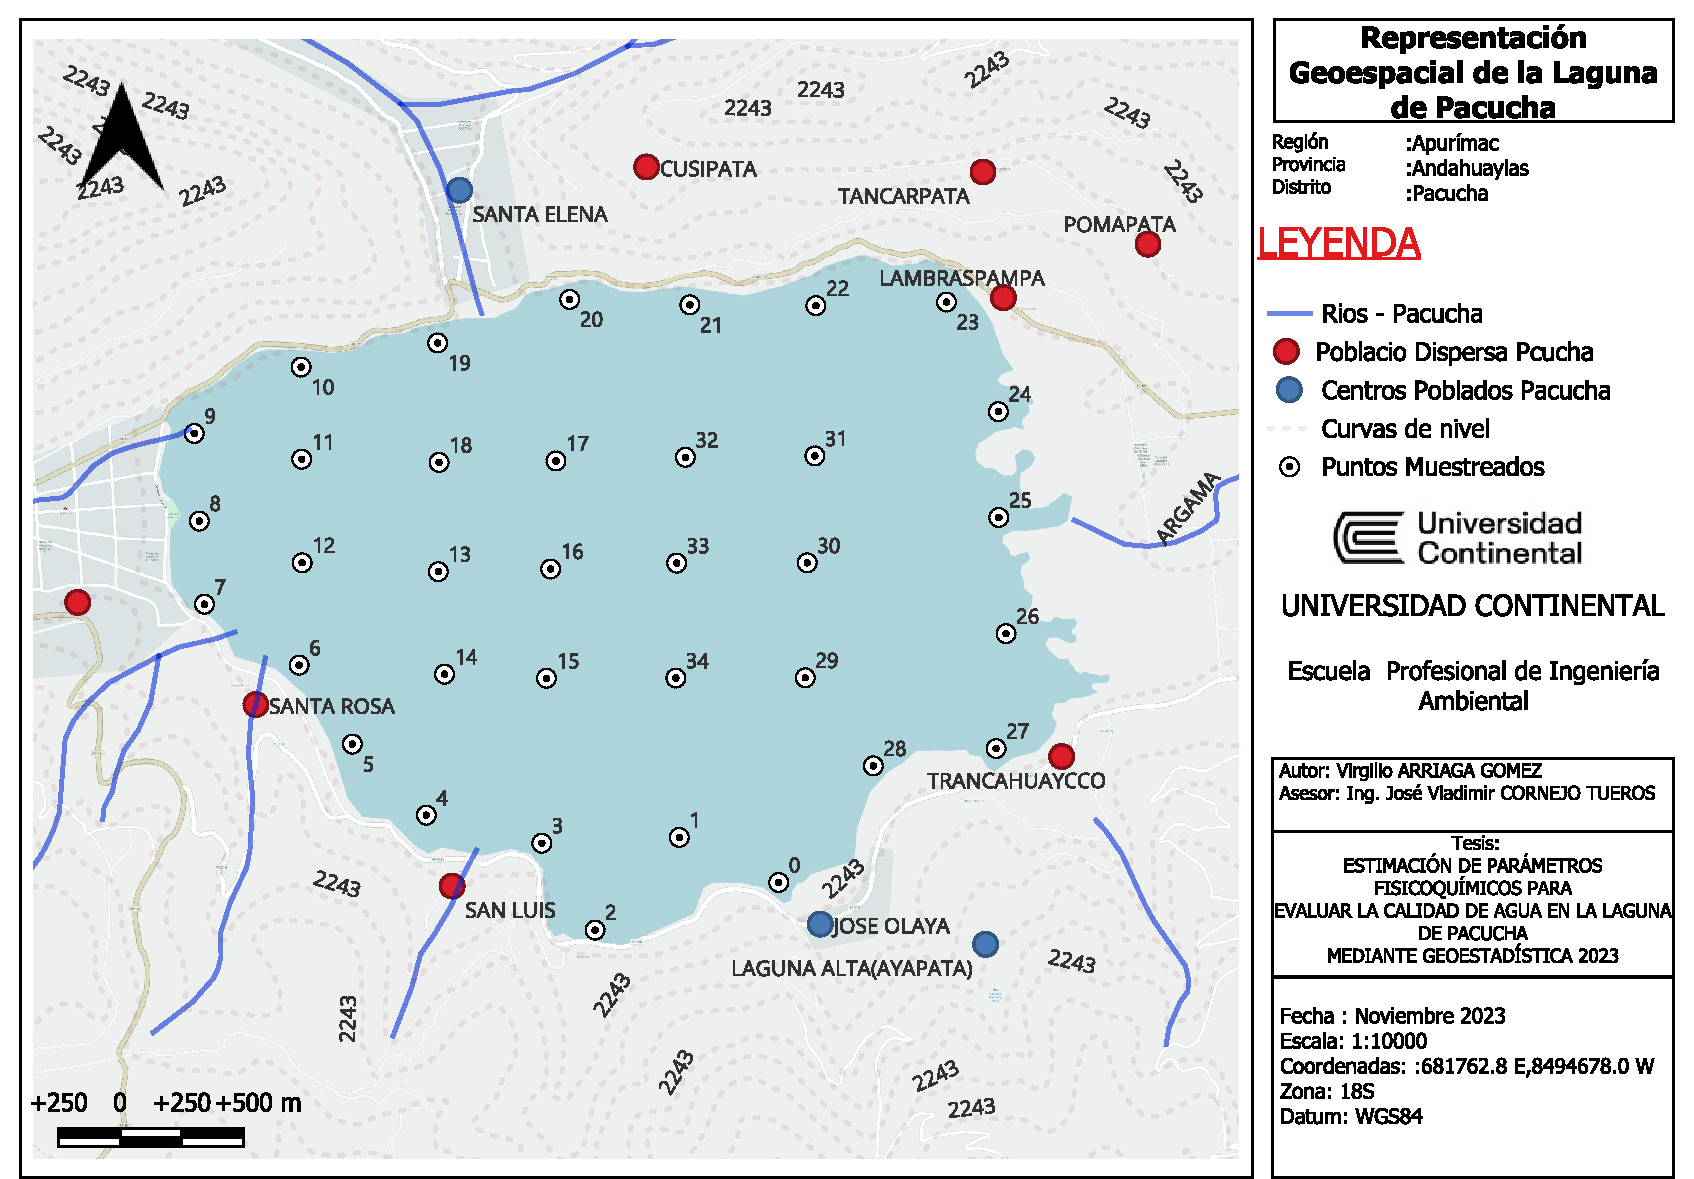
\includegraphics[width=0.9\linewidth]{Capitulos/GEOESTADICTICA_PACUCHA.pdf} 
        \caption{Mapa de la Laguna de Pacucha} % Agrega un título a la imagen.
    \end{figure}
\end{landscape}


